\chapter{Background}

This chapter discuss historical researches and describes main concepts and terminologies used through out this thesis.
It covers mainly topic about \gls{ai} and \gls{ml}.

\section{Artificial Intelligence and Machine Learning}

% Philosophy and Psychology

Terms like ``Intelligence'', ``Knowledge'', ``Thinking'' and ``Learning''
have been controversial for long time. In 1950, Alan Turing proposed the question ``Can machines think?''\autocite{machinery1950computing}.
and instead of trying to answer that question, he proposed using a behavioral test for intelligence in what he called ``imitation game''.

Human intelligence is manifested in many abilities like the ability to plan, solve problems, make decisions,
perceive information, retain knowledge, comprehend ideas, reason, form concepts, recognize patterns,
involving cognition, motivation, feelings (emotional knowledge), and self-awareness.
Learning, thinking, and communication using languages.

This research focus on one of those abilities which is the ability to recognize images.

\gls{ai} is usually defined using the paradigm of intelligent agent

\begin{quote}
``Any device that perceives its environment and takes actions that maximize its chance of success at some goal.'' \autocite{russell2003artificial}
\end{quote}

And for such agent to be able to learn, here comes the need for \gls{ml}

\begin{quote}
``Machine learning involves adaptive mechanisms that enable computers
to learn from experience, learn by example and learn by analogy.
Learning capabilities can improve the performance of an intelligent system over
time. Machine learning mechanisms form the basis for adaptive systems.''\autocite{michael2005artificial}
\end{quote}

A computer program is said\autocite{thrun1998learning} to ``learn'' if its performance at the task improves with experience.
This means we need to define a performance metric and a way to pass examples to it, giving it experience.
This process is called training. The metric to be minimized can be called error, loss, cost, ..etc or
to be maximized like fitness, reward, profit,... etc..

Humans do multiple learning tasks (concepts, skills, ..etc.) simultaneously where knowledge flows as a stream.
Beside learning such tasks, they learn how to learn and how to generalize even if only given a single example. 
On the other hand, known ``Machine Learning'' techniques require many examples (sometimes in thousands)
and the domain(s) and task(s) are fixed (translate from English to Arabic, diagnose cancer or drive an autonomous car).

If the examples passed to the machine are labeled (those are examples of dogs, and those are cats),
then the task is called a ``supervised'' task.
If the examples are not labeled, then the task is called ``unsupervised'', 
(given those loads of cats and dogs pictures, let's put them apart, without knowing which is which)
``Semi-supervised learning'' is very similar to ``supervised learning'' having a small number of labeled examples,
and loads of unlabeled examples.



\section{Classification Tasks}

This research discuss one of the common \gls{ml} applications, which is ``classification''.
Given a classification task \( \tau \) belonging to some specific domain \( D \) in some specific feature space \( \chi \)
having instances like \( X \) in the form \( \{x_1, x_2, ..., x_n \} \),
having marginal probability distribution \( P(X) \) for every \( X \in \chi \), 
and label space \( Y \)

\begin{equation}\label{eq_domain}
D = \{ \chi , P(X) ; X \in \chi \}
\end{equation}

and given a labeled training dataset \( T = \{ (X_1, y_1), (X_2, y_2), ... \} \),
for \( X_i \in \chi \), \( y_i \in Y \).

The classification task is defined\autocite{pan2010survey} to find a function \( g(X) \) that predicts the label
having maximum conditional probability \( P(y|x) \) 
or predict the joint probability of each label \( f(X,y) = P(X,y) \) in the domain

\begin{equation}\label{eq_task}
\tau = \{ Y , P(y|X) ; y \in Y \}
\end{equation}

There are two main types of supervised classification tasks:
``Constructive models'' (like ``Generative Models'') and ``Discriminative Models''.
Constructive models tries to understand how the output is generated from the input,
as in the case of Generative Models\autocite{battiti2017lion} try to model how a class \(y\) relates to input \(x\)
in the form of class-conditional density\(p(y_{0}|x)\) as in by Bayes’ theorem \ref{eq:y_given_x}.

\begin{equation}
p(y_{0}|x) = \frac { p(x|y_{0}) \cdot p(y_{0}) } { \sum\limits_{y} p(x|y) \cdot p(y) }
\label{eq:y_given_x}
\end{equation}

Where \(p(y_0)\) is the prior probability, and \(p(x|y_0)\) is the likelihood of the data.
The denominator normalize the formula to make it sum into one.
Which means that it needs to model \(p(x|y_{0})\).

Discriminative models, on the other hand, only care about the end result of the classification
without knowing the relation that forms different instances \(x\) in a given class \(y0\).


A binary classifier is a classifier that has two labels or classes (that is \(Y\) has two members),
it's either a yes or no, a cat or dog, if it's not a dog then it's a cat (no none).
the probability of one is complementary to the other \( P(y2)=1-P(y1) \).

\begin{itemize}
\item ``does the given input data indicate that this patient has Diabetes? yes or no''
\item ``is this a picture of a dog? yes or no'' (or equivalently ``is this a dog or a cat?'')
\end{itemize}

There are different ways to implement a binary classifier 
like the original \gls{svm} paper\autocite{cortes1995support}
or as a neuron with only one output (that either activated or not activated).

Multi-class classifier have more than two members in \(Y\), let's say a cat, a dog or a bird.
There are two strategies to extend a binary classifier like the original \gls{svm}
into multi-class classifier\autocite{vapnik1995nature}\autocite{hsu2002comparison}\autocite{knerr1990single}

\begin{description}
\item [``one against one''] - performing pair-wise comparisons between all \(n\) classes
\item [``one against all/rest''] - perform comparisons against all at once, not pair-wise.
\end{description}

Here are some examples of classification tasks and their data sets

\begin{description}
\item [Fisher's  Iris Flower data set] - has three classes ``Setosa'', ``Versicolour'', and ``Virginica''
based on four features that is Petal length, Petal width, Sepal length, and Sepal length\autocite{fisher1936use}.
\item [Breast Cancer Wisconsin (Diagnostic) Database] - has two labels (Malignant and Benign)
and 30 numeric attributes\autocite{street1993nuclear}\autocite{wolberg1994machine}\autocite{mangasarian1995breast}.
\end{description}

\section{Knowledge Transfer}\label{transfer}

Given a trained model for some task (an accurate solved problem),
and a another different but similar task that is to be addressed (unsolved problem).
``Knowledge Transfer'' is all about reusing the source task to solve the target task.
There are many different approaches for doing this some (like Category Adaptation)
does not involve training target task while others use transfer only as an initialization
and require training target task.


\section{Domain-specific Image Recognition}

Domain-specific Image Recognition application as in ``Face recognition'' and ``Fingerprint scanner'',
not only utilize specialized algorithms that are only valid in that domain but also typically work
on pre-processed images so that images are centered, segmented and have fixed orientation.

\section{Artificial Neural Networks}

The most basic form of \gls{ann} or simply \gls{nn} is ``Perceptron'',
which is basically one output that is the result of weighted summations of
all inputs plus some scalar value called ``bias'' then apply some function that is called ``activation function''
to achieve non-linearity.

Slightely more complex \gls{ann} have more than one output, having different weights and bias values for each output.
For example, in figure \ref{fig:ann1} \(o_1\) is the weighted summation of \(i_1\), \(i_2\), \(i_3\), and \(i_4\) that is
\( o_1 = F(w_{11}\cdot i_1 + w_{12}\cdot i_2 + w_{13}\cdot i_3 + w_{14}\cdot i_4) \).

\begin{figure}[!ht]
\centering
    \begin{subfigure}[b]{0.48\textwidth}
        \centering
        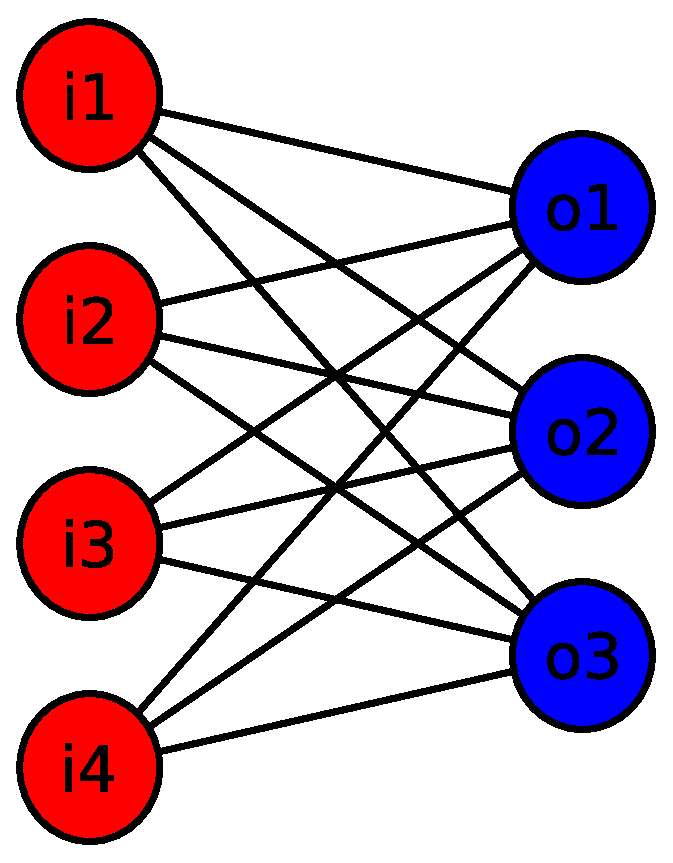
\includegraphics[width=0.7\textwidth]{ann1}
        \caption{A simple neural network with single layer that is the output layer of size three output nodes formed from four input layers and no hidden layer}\label{fig:ann1}
    \end{subfigure}
    \begin{subfigure}[b]{0.48\textwidth}
        \centering
        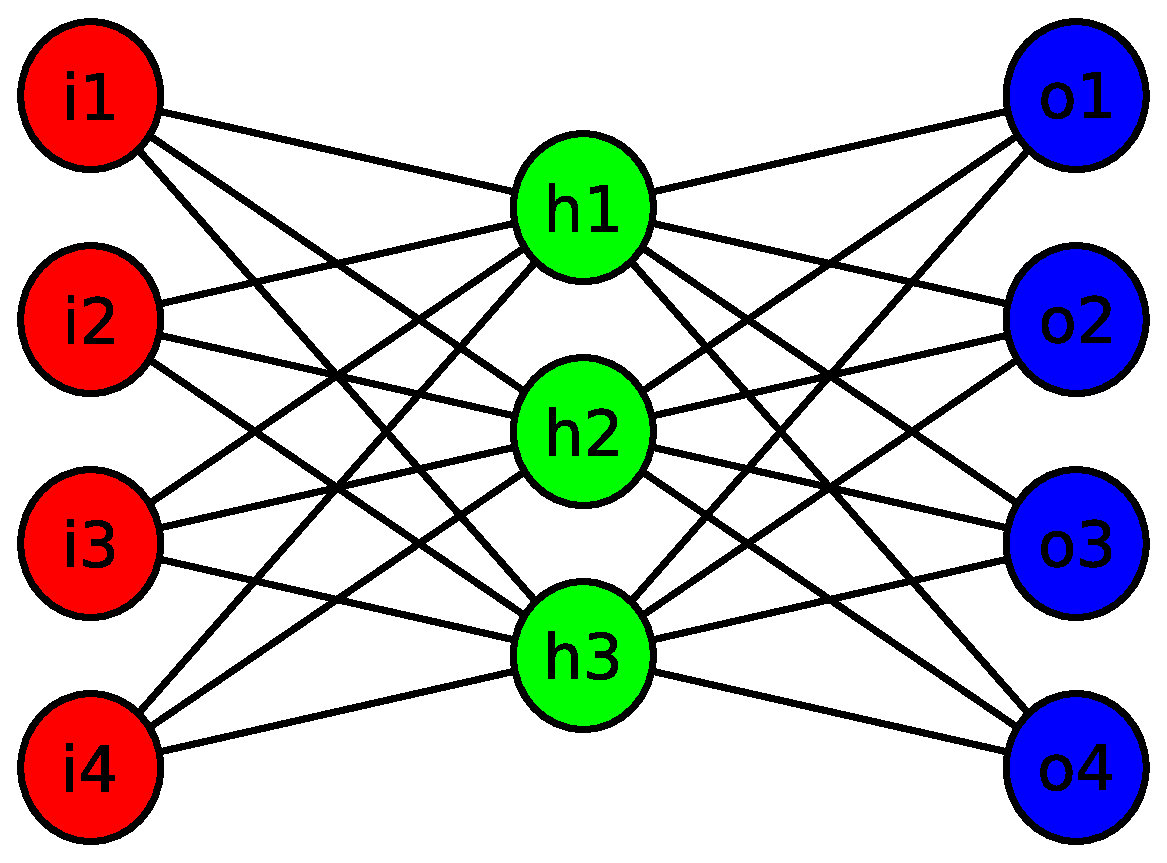
\includegraphics[width=\textwidth]{ann2}
        \caption{A neural network with a single hidden layer of size three between four input nodes and four nodes outputs}\label{fig:ann2}
    \end{subfigure}
\caption{Two simple neural networks, input in red, output in blue.}\label{fig:ann}
\end{figure}


The weighted summation can be expressed in the form of matrix multiplication.
That is given input \(I\) of size \(n\) written as \(I_{n\times 1}\),
output of size \(m\) written as \(O_{m\times 1}\),
the weights \(W_{m\times n}\), and bias values \( B_{m\times 1} \), and activation function \( F \)
The output of the perceptron is defined by formula \ref{eq:perceptron}

\begin{equation}
O_{m\times 1} = F( W_{m\times n} \times I_{n\times 1} + B_{m\times 1} )
\label{eq:perceptron}
\end{equation}

The most basic form of activation function \(F(x)\) is a simple threshold as in \ref{eq:relu} denoted as \( [x]^+ \),
if the weighted summation plus the bias is greater than zero, it's kept as is (activated),
otherwise it's zero (deactivated). The value of the bias controls the threshold.
This form of activation function is called
\gls{relu}\autocite{hahnloser2001permitted}\autocite{jarrett2009best}\autocite{nair2010rectified}

\begin{equation}
f( x ) = [ x ]^+ = max(0, x)
\label{eq:relu}
\end{equation}

There exist many other forms of activation functions like ``Sigmoid functions''\autocite{orr1998neural}\autocite{lecuniefficient}

\begin{equation}
f( x ) = \frac{ 1 }{ 1+e^{-x} }
\label{eq:tanh}
\end{equation}

\begin{equation}
f( x ) = \tanh(x)
\label{eq:tanh}
\end{equation}

\begin{equation}
f( x ) = \tanh(x) + a\cdot x
\label{eq:tanh_plus_linear}
\end{equation}

A common setting for ``Scaled hyperbolic tangent''\autocite{lecun1989generalization} in \ref{eq:scaled_tanh}
is to have \(A=1.7159\) and \(S=2/3\), which would result \(f(1)=1\) and \(f(-1)=-1\).

\begin{eqfloat}
\begin{equation}
f( x ) = A \cdot \tanh(S\cdot x)
\label{eq:scaled_tanh}
\end{equation}
\caption{Scaled hyperbolic tangent. Source:\autocite{lecun1989generalization}}
\end{eqfloat}

A multi-layer neural network is merely a concatenation of simple ones,
the neural network first generate an intermediate state
called hidden layer, then that hidden layer is then become an input of another stage as seen in figure \ref{fig:ann2}.
One can add many intermediate hidden layers.
``Deep Neural Network'' is that with more than one hidden layer.
 
The training process is composed of two phases, forward pass (or forward propagation), and ``Back propagation''.
Parameters (weights and bias values) are randomly initialized, then in forward pass,
each input instance is passed through the \gls{ann}, and compared against the desired output
using some cost function like mean squared error \(E\)
and used to adjust weights accordingly as in figure \ref{fig:bp},
that's why training process is a form of optimization problems with objective to minimize the cost function.

\begin{figure}[!h]
\centering
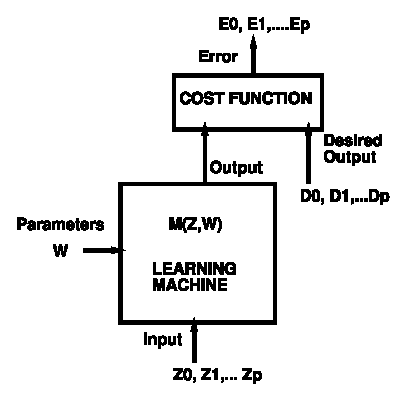
\includegraphics[width=2in]{bp}
\caption{Gradient based learning.}\label{fig:bp}
{Source: \autocite{lecuniefficient}\autocite{orr1998neural}\hfill}
\end{figure}

When having \(n\) layers, the input is denoted as \(X_0\),
the output of first hidden layer is \(X_1\), the last output of the whole network is \(X_n\).
Output can be expressed as a recursive formula \ref{eq:ann_ouput} as in\autocite{lecuniefficient}\autocite{orr1998neural}

\begin{equation}
X_n = F_n(W_n, X_{n-1})
\label{eq:ann_ouput}
\end{equation}

Typically \(F_n\) is the activation function applied to the matrix multiplication of weights to input.

\begin{equation}
X_n = sigmoid( W_n \times X_{n-1}) )
\label{eq:ann_as_matrix}
\end{equation}

\begin{equation}
y = X_n
\end{equation}

\begin{equation}
E = \frac{1}{2} \sqrt{ ( y_{d} - y )^2 }
\end{equation}

A fraction of difference between the desired result and the obtained result is carried backward
(thus the name ``Back propagation'') to adjust the weights,
that fraction is called ``Learning Rate'' in \ref{eq:weights_update} it's \(\eta\)
which can be a constant like 0.01 or some faded value through out the process.
This process is called ``gradient descent''.

\begin{equation}
W(t) = W(t-1) - \eta \cdot \frac{\partial E}{\partial W}
\label{eq:weights_update}
\end{equation}

\begin{equation}
\Delta W = - \eta \cdot \frac{\partial E}{\partial W}
\end{equation}

Taking a random instance (or a very small random subset of training data)
at each step then this is called \gls{sgd}.
Streaming instances and doing the update as they come is called ``online learning''.

\section{Neural Networks for Classification}\label{sec_nn_classification}

Taking the classical example of Iris database, which have four input features
and a corresponding label that has three possible values.
Each one of the three possible classes is made into an output node in the neural network,
and ``Hot One Encoding'' is used to represent it, like this:

\begin{enumerate}
\item ``Setosa'' is represented as \( \begin{bmatrix}1 & 0 & 0\end{bmatrix}^T \)
\item ``Versicolour'' is represented as \( \begin{bmatrix}0 & 1 & 0\end{bmatrix}^T \)
\item ``Virginica'' is represented as \( \begin{bmatrix}0 & 0 & 1\end{bmatrix}^T \)
\end{enumerate}

Only one output node is activated that correspond to the desired class/label.

Normalized exponential function (Softmax)\ref{eq:softmax} is used to convert the open-ended actual output
into probability-like output, because softmax has to important properties\autocite{nasrabadi2007pattern}

\begin{itemize}
\item each output in the interval [0, 1]
\item the summation of all output values is 1.
\end{itemize}

\begin{equation}
softmax(o_j) = \frac{e^{o_j}}{ \sum\limits_{i=1}^n e^{o_i} }
\label{eq:softmax}
\end{equation}

One problem of this, is that it would boost otherwise negligible values as it has to make the summation equal to 1,
for example, given two output nodes having 0.01 and 0.001 the softmax will map them into 50.2\% and 49.8\%.
When given a picture of a tree in a cat or dog task, the probability of being a cat or being a dog
would always be high, it's either a cat or a dog, it would never return a number smaller than some threshold
indicating none of them.

\section{Generalization}

If one made a ML learning model that memorize all the training dataset,
then it would be wrongly considered accurate as it would fail to generalize
and when presented with input that was not part of training data it would fail miserably
this is called ``Over-fitting''.
To measure this, part of the dataset is put aside into ``test dataset''
that is never presented during training but rather used later to evaluate the model.

In case of mini batches with \gls{sgd}, each small batch is also shuffled and split into training and validating dataset.

Regularization\autocite{ng2004feature} tend to prefer smaller weights like the green curve in figure \ref{fig:regularization},
by adding a scalar multiple of weights magnitude summation to the loss function, either absolute value as in ``L1 Regularization''\ref{eq:l1}
or squared as in ``L2 Regularization''\ref{eq:l2} or both\ref{eq:l12}. The scaler \(\lambda\) is called ``Regularization Penalty''.


\begin{equation}
C_{l1} = C + \lambda \sum\limits_{i} | w_i |
\label{eq:l1}
\end{equation}

\begin{equation}
C_{l2} = C + \lambda \sum\limits_{i} w_i^2
\label{eq:l2}
\end{equation}

\begin{equation}
C_{l12} = C + \lambda_1 \sum\limits_{i} | w_i | + \lambda_2 \sum\limits_{i} w_i^2
\label{eq:l12}
\end{equation}


\begin{figure}[!h]
\centering
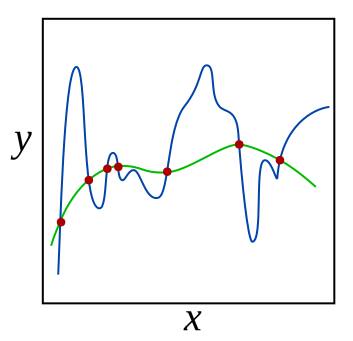
\includegraphics[width=2in]{regularization}
\caption{Two curves that have same loss of zero. Green one have smaller weights, blue one have higher weights. }\label{fig:regularization}
{Source: \href{https://commons.wikimedia.org/wiki/File:Regularization.svg}{Wikipedia}\hfill}
\end{figure}

Another method to force the neural network to generalize is to introduce noise in the training dataset.
Another method is to randomly drop parts of the signal, which is called ``dropout layer''

\section{Convolutional Neural Networks}

\gls{cnn} or more commonly ConvNets was inspired by how
visual cortex is assumed to work. \gls{cnn} is similar to \gls{ann} but uses Convolutional Matrix operator.
The 3D volume formed by multiple 2D matrices channels is called a ``Tensor'',
Given an input image in the form of a Tensor formed by of multiple 2D matrices of pixels for each color channels,
several filters can be written in the form of convolution matrix like edge detection (as in figure \ref{fig:conv-edge}),
sharpen, smoothing/blurring (as in figure \ref{fig:conv-blur}), and pattern matching.
\gls{ann} can be used to learn the values in many convolutional matrices resulting in image filters that
activate when being exposed on specific visual features or structures.

End-to-End solutions feed unprocessed input directly without much prepossessing (if any at all)
and get the end desired result and \gls{nn} is good at that.

The size of each convolutional filter matrix which is also called the ``kernel size'' or the ``neighborhood size''
specifies the receptive field of the filter.
For example, a kernel of size 3×3 means that bounding box of neighborhood starts one pixel to left, one pixel to top
and ends on one pixel to the right and one pixel to the bottom while 5×5 kernel size means two pixels neighborhood
from each side. 

\begin{figure}[!htbp]
\centering
    \begin{subfigure}[b]{0.32\textwidth}
        \centering
\[
\begin{bmatrix}
0 & -1 & 0 \\
-1 & +4 & -1 \\
0 & -1 & 0 
\end{bmatrix}
\]
    \end{subfigure}
    \begin{subfigure}[b]{0.32\textwidth}
        \centering
        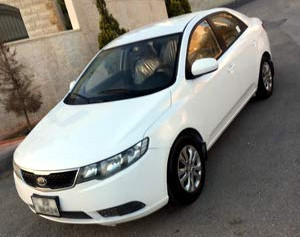
\includegraphics[width=\textwidth]{car}
    \end{subfigure}
    \begin{subfigure}[b]{0.32\textwidth}
        \centering
        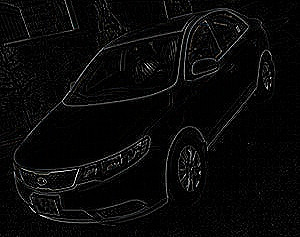
\includegraphics[width=\textwidth]{car-conv-edge}
    \end{subfigure}
\caption{Laplacian operator (edge detection) written as 3×3 convolutional matrix}\label{fig:conv-edge}
\end{figure}

\begin{figure}[!ht]
\centering
    \begin{subfigure}[b]{0.32\textwidth}
        \centering
\[ \begin{aligned}
\frac{1}{16}\cdot
\begin{bmatrix}
1 & 2 & 1 \\
2 & 4 & 2 \\
1 & 2 & 1 \\
\end{bmatrix}
\end{aligned} \]
    \end{subfigure}
    \begin{subfigure}[b]{0.64\textwidth}
        \centering
        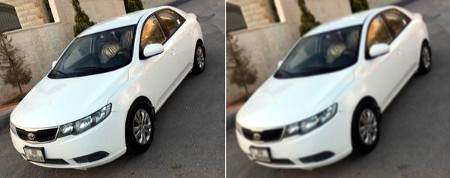
\includegraphics[width=\textwidth]{car-blurred}
    \end{subfigure}
\caption{A blur filter written as 3×3 convolutional matrix}\label{fig:conv-blur}
\end{figure}

The convolution operator used in \gls{cnn} is called 2D convolution
(usually named ``conv2d()'' or ``conv\_2d()'' depending on the used software package)
and it operates on 3D volumes (taking a 3D volume as input and resulting a 3D volume as output)
For example, an input can be a colored image of size 224×224 and depth of 3 RGB channels
(written as \(224×224×3\) or \(3@224×224\)\autocite{lecun1998gradient}),
when passed to a convolution on a neighborhood size 3×3 and depth of 96 channels (written as \(3×3×96\) or \(96@3×3\))
result would be an output volume of size 224×224 (or 222×222 in case of no padding) and depth of 96.
The size of the input is \(width\times height \times depth\) or for short \(W_i\times H_i\times D_i\).
And the output size is \(W_o\times H_o\times D_o\).
The depth of the convolution kernel represent how many filters do we want to apply/learn.

Gray-scale images have input depth of one, but even in that case we still need to operate in 3D volumes,
because we don't want to learn a single filter, after first convolution we would have an output of 3 axis.

Convolution depth varies from layer to layer but input depth of
a layer must match output depth of the previous layer as they work in a pipeline.

So passing an image of size \( W_i\times H_i \) and input depth \( D_i \) (ex. \( D_i=3 \) for RGB channels)
to a convolution layer of kernel size \(W_k\times H_k\) and output depth \(D_o\) would have number of weights
to be learned is \( W_k\times H_k \times D_o \times D_i \) plus \(D_o\) bias values.

You can think of convolution layers as an operator that takes a 3D volume of \(W_i\times H_i\times D_i\)
and result a 3D volume of \(W_i\times H_i\times D_i\) and this operator is to be applied to every possible pixel
in the image by starting from top-left corner (in case of padding), where the neighborhood window is centered,
and slide that window one pixel until all input image is covered. 

In summary a convolution layer has the following properties:

\begin{description}
\item [Input volume size:] \(W_i\times H_i\times D_i \)
\item [Kernel size:] \( W_k\times H_k\times D_o \)
\item [Output volume size:] \( W_o\times H_o\times D_o = W_i\times H_i\times D_o \)
\item [Number of parameters:] are
\begin{itemize}
\item \( W_k\times H_k\times D_o\times D_i \) weight values
\item \( D_o \) bias values
\end{itemize}
\item [Number of window positions:] \( P = W_o\times H_o \)
\item [Number of multiplications in a given position:] \( W_k\times H_k\times D_o\times D_i \)
\item [Number of addition operations in a given position:] \( W_k\times H_k\times D_i\times D_i\) (and another one for bias)
\item [Total number of multiplication operations] \( W_o\times H_o\times W_k\times H_k\times D_o\times D_i\) and same value for addition operations
\end{description}

In case of no padding, convolution start at offset \( =\frac{W_k-1}{2} \) pixels (and a similar offset to the end)
which would be make output smaller by \(W_k-1\) that is \(W_{i}-W_{k}+1\) so with height.

The final objective of all convective convolution operators after all layers of any CNN is
to get us to the desired labels of the classification task, that is \(D_o\)
of the last layer is either the labels or flat features that are being fed to usual \gls{ann} (called Fully Connected layers).

An important special case of no-padding convolution is the case when kernel size matches input size,
that is \(W_i=W_k\) then the output width would be \(W_{i}-W_{k}+1=W_i-W_i+1=1\),
similarly with the height, then the size of the output would be 1×1.
Which converts the 3D volume into one dimension along the depth,
making it suitable to be considered to correspond to the desired labels in the classification task or
to flat features to be fed to usual \gls{ann}.

Another important note that 1×1 convolution with depth \(D_o\)
have the same effect of a hidden layer of size \(D_o\) in usual \gls{ann}.

\begin{itemize}
\item Input volume size: \(1 \times 1 \times D_i \)
\item Output volume size: \( 1 \times 1 \times D_o \)
\item Number of parameters:
    \begin{itemize}
    \item \( D_i \times D_o \) weight values
    \item \( D_o \) bias values
    \end{itemize}
\item Number of window positions: \( P = 1 \times 1 = 1 \)
\item Total number of multiplication operations = \( D_i\times D_o \) and same value for addition operations
\end{itemize}

Some designs may involve sliding more than one pixel at a time, which is a hyper-parameter called ``Stride''
and usually written as \(/S\), for example a kernel of \(5×5×96/3\) means it has width and height of five,
depth of 96 and stride of 3.
And it's a technique used to reduce number of operators (but it does not reduce number of weights).
With a stride value of two output width and height halves. With a Stride of one it's like having no stride.

\begin{description}
\item [Input volume size:] \( W_i\times H_i\times D_i \)
\item [Kernel size:] \( W_k\times H_k\times D_o / S \)
\item [Output volume size:] \( \frac{W_i}{S} \times \frac{H_i}{S} \times D_o \)
\item [Number of parameters:] are
\begin{itemize}
\item \(W_k\times H_k\times D_o\times D_i \) weight values
\item \(D_o\) bias values
\end{itemize}
\item [Number of window positions:] \( P = W_i\times H_i / S^2 = W_o\times H_o \)
\item [Number of multiplications in a given position:] \( W_k\times H_k\times D_o \times D_i \)
\item [Number of addition operations in a given position:] \( W_k\times H_k\times D_i\times D_o\) (including one for bias)
\item [Total number of multiplication operations:] \(W_o\times H_o\times W_k\times H_k\times D_o\times D_i \) and same value for addition operations
\end{description}

The effect of stride is not limited to reducing number of multi-add operations but on the exponential
effect of reducing the output volume of this filter becoming input filter of next layers, for example
applying five layers of convolution with stride of two would reduce width and height of 224×224 into 7×7, because \(224/(2^5)=7\).

\section{No weights layers}

In CNN, not all layer have weights.
Pooling layers have a neighborhood window size and a stride \(S\) written as \(W_k\times H_k / S\).
It uses some aggregate operator like maximum or average to summarize the signal in that window,
that is moved \(S\) pixels each time, resulting on a down-sampled image.
For example average pooling of size 2×2 and stride of 2 (written as 2×2/2)
would have the effect of down-sampling the input image by factor 2.
Pooling is possible with window size not matching the stride,
and is also possible without stride at all (\(S=1\))
that is to summarize surrounding input signals in the window.

The difference of applying stride in convolution or in a pooling layer after it,
is that the first one ignores some input signals while the other one takes the strongest signal (in case of max-pooling).

Another form of no-weights layers is to apply some activation function on input like ``Rectifier Layer''
which applies \gls{relu}\autocite{hahnloser2001permitted}\autocite{jarrett2009best}\autocite{nair2010rectified} to input as in formula \ref{eq:relu}.
Such layers does not affect the shape of its input volume.

\section{Design of CNN models}

A typical basic design of a \gls{cnn} model starts with an input image of certain width and height \(W_{i}\times H_{i}\)
in case of colored images that is a volume of size \(W_{i}\times H_{i}\times 3\).
Then that volume is feed to a sequence of convolution layers of certain kernel size and depth (number of filters).
Then comes a pooling layer (maximum pooling or average pooling), then that is repeated alternating convolution and pooling layers.

The objective of the design is to form a flat signal of no spacial dimension (width=1 and height=1)
but rather along the depth which will be the signal of output classes.
To reduce the width and the height of the signal volume, stride is used on convolution layer or pooling layers.
Different designs of CNN models use stride at different stages, it can be placed early,
down-sampling the signal too early will trade accuracy with speed.

Toward end of the model, either pooling or convolution of kernel size
matching the size of the input will summarize the signal into the desired flat signal of size \(1\times 1\).
When the signal is flat along the depth (having width and height equal to one),
classical \gls{ann} can be used, this is called fully connected layers,
this is equivalent of convolution of kernel size \(1\times 1\).

The last signal is processed with Softmax function as in equation \ref{eq:softmax} to make output signal
form probabilistic-like values as previously discussed in section \ref{sec_nn_classification}.

Figure \ref{fig:cnn-flowchart} shows the whole process of such design.

\begin{figure}[!ht]
\centering
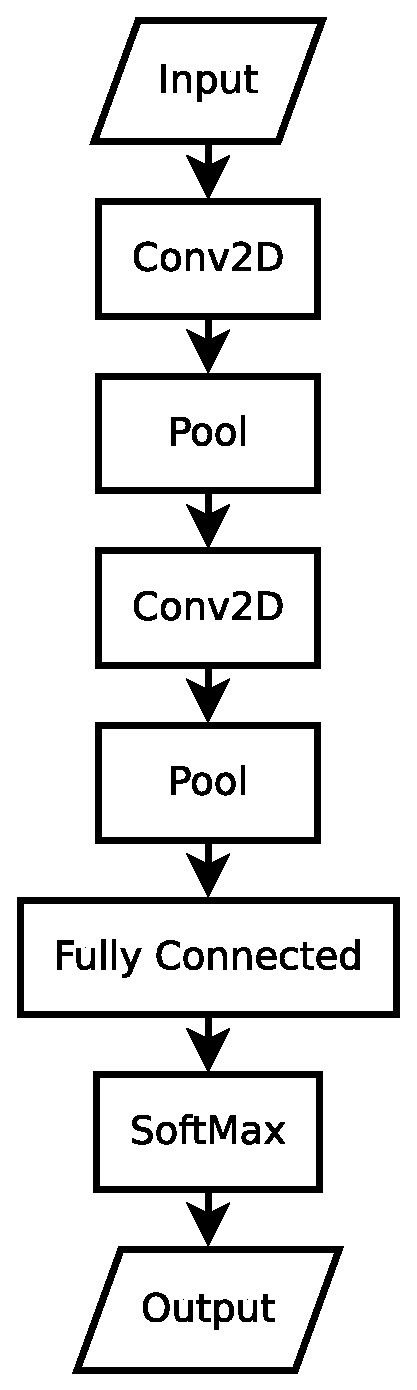
\includegraphics[width=2in]{cnn-flowchart}
\caption{A simple CNN design.}\label{fig:cnn-flowchart}
\end{figure}


\section{Batch Normalization Layers}

Just like it's important to normalize input signal (for example, by subtracting mean and dividing by variance),
it's also important to regulate hidden layers signals.
A batch normalization layer\autocite{ioffe2015batch} is placed after some hidden layers,
having two trainable parameters that are called ``scale'' and ``shift'',
which is updated for each mini-batch in training phase, by finding batch mean and variance.

Some researches suggest using larger mini-batches\autocite{goyal2017accurate}.

\section{Separable Operators}

One of the methods used to reduce number of weights is to decompose the kernel from
being of size \( n \times m \) into two matrices of size \( n \times d \) and \( d \times m \)
and typically \( d=1 \), in this case the number of weights would be
\( (n\times 1)+(1\times m)=n+m\) instead of \(n\times m\)
(or \(2 \cdot n\) instead of \(n^2\) when width and height are equal).
For example one can write a \(3\times 3\) blur kernel using
two matrix multiplication of size \(3\times 1\) and \(1\times 3\) as in (\ref{eq:sep_blur}),
there are a total of six weights in two matrices (3×1 and 1×3) compared to nine in the equivalent 3×3 matrix.

\begin{eqfloat}
\begin{equation}
\begin{bmatrix}
1 \\
2 \\
1
\end{bmatrix}
\times
\begin{bmatrix}
1 & 2 & 1
\end{bmatrix}
=\begin{bmatrix}
1 & 2 & 1 \\
2 & 4 & 2 \\
1 & 2 & 1 \\
\end{bmatrix}
\label{eq:sep_blur}
\end{equation}
\caption{ 3×3 blur operator written as two matrices each of three }
\end{eqfloat}

Beside being used along the width and height of the convolution kernel it can be used along kernel depth
where the convolution kernel of \( W_k \times H_k \) that takes input of depth \(D_i\)
and output depth of \(D_o\) using intermediate value called depth multiplayer \(D_M\) and which can be 1.
One way of doing this is two consecutive convolutions one is called\autocite{chollet2016xception}\autocite{mamalet2012simplifying}
``depth-wise convolution'' that operate on a kernel of 3×3 on an intermediate depth of \(D_M\) (typically 1)
and the other is called ``point-wise convolution'' that operate on a kernel of 1×1 with output depth of \(D_o\)

\newcommand{\ra}[1]{\renewcommand{\arraystretch}{#1}}

\begin{table*}\caption{How separable operators reduce number of weights and multiplications}\label{table:sep_op}
\centering
\begin{small}
\begin{tabularx}{\textwidth}{cccccrX}
\toprule
Name & Input & depth & kernel & depth & weights & mults \\
\midrule
original & 224×224 & 3 & 3×3 & 96 & 3×3×3×96 =2,592 & 224×224×3×3×3×96 = 130.1M \\
\bottomrule
\multicolumn{7}{c}{Separable equivalent} \\
\midrule
depth-wise & 224×224 & 3 & 3×3 & 1 & 3×3×3×1 =27 & 224×224×3×3×3×1 =1.4M \\
\midrule
point-wise & 224×224 & 1 & 1×1 & 96 & 1×1×1×96 =96 & 224×224×1×1×1×96 =4.8M \\
\cmidrule{5-7}
\multicolumn{5}{r}{Total} & 27+96 =123 & 6.2M \\
\bottomrule
\end{tabularx}
\end{small}
\end{table*}

\begin{table*}\caption{Separable operators reduction applied to hidden layer}\label{table:sep_hidden}
\centering
\begin{small}
\begin{tabularx}{\textwidth}{cccccrX}
\toprule
Name & Input & depth & kernel & depth & weights & mults \\
\midrule
original & 224×224 & 64 & 3×3 & 64 & 64×3×3×64 =36,864 & 224×224×64×3×3×64 =1,849.7M \\
\bottomrule
\multicolumn{7}{c}{Separable equivalent of same hidden layer} \\
\midrule
depth-wise & 224×224 & 64 & 3×3 & 1 & 64×3×3×1 =576 & 224×224×64×3×3×1 =28.9M \\
\midrule
point-wise & 224×224 & 1 & 1×1 & 64 & 1×1×1×64 =64 & 224×224×1×1×1×64 =3.2M \\
\cmidrule{5-7}
\multicolumn{5}{r}{Total} & 640 & 32.1M \\
\bottomrule
\end{tabularx}
\end{small}
\end{table*}

As we can see table \ref{table:sep_op} when have an input image of size 224×224 and 3 RGB channels
which is convolved with 3×3 kernel and 96 filters (output depth),
then typically we have 2.5K weights and 130M multiplications.
A separable counterpart of 3×3×1 and 1×1×96 with same input volume
and output volume would have only 123 weights and 6M weights.
In the second case as in table \ref{table:sep_hidden} when we take an input volume of size 224×224×64 to be convolved with a kernel of 3×3
and an output depth of 64, the usual convolution have 36K weights and 1,800M multiplications.
On the other hand the separable version of \(D_M=1\) have only 640 weights and 32M multiplications.

\section{Accuracy Metrics}

\begin{description}
\item [Accuracy rate] which is the ratio of true items, both true positives (\(T_P\))
and true negatives (\(T_N\)) over total (or its complement ``Error rate'' which is the ratio of false items both
false positives \(F_P\) and false negatives \(F_N\) over total).
Those two metrics are vulnerable if the likelihood of labels are not equal.
For example, if the problem domain is diagnosing cancer,
assuming that the probability of cancer is small like 0.1\%,
a classifier that randomly pick cancer positives with very small probability or even not report any cancer positive at all
(classify every body as healthy) would have very high accuracy (99.9\%)
and low error rate (since it only mistaken people with cancer, so it have error rate of 0.1\%).
To overcome this, a metric (like ``Precision'' and ``Recall'' below) is needed
that does not consider success rate or failure compared
to total, but makes the denominator to be limited to smaller context.  
\begin{equation}
Accuracy = \frac{ T_P + T_N}{ SampleSize }
\label{eq:precision}
\end{equation}
\item [Precision] is the ratio of true positive items over positively diagnosed items (both \(T_P\) and \(F_P\)),
which is a measure of Type I error caused by the \(F_P\) in the denominator \ref{eq:precision}.
\begin{equation}
Precision = \frac{ T_P }{ T_P + F_P }
\label{eq:precision}
\end{equation}
\item [Recall] is the ratio of true positive items compared all positive items
(both truly diagnosed and falsely missed), which is a measure of Type II error that cases the \(F_N\) in the denominator \ref{eq:recall}.
\begin{equation}
Recall = \frac{ T_P }{ T_P + F_N }
\label{eq:recall}
\end{equation}
\end{description}

In the above example of random cancer diagnose that picks 0.1\%, in a sample of 10,000 person,
it would randomly diagnose ten persons with cancer, but only one of them actually have cancer
and it missed eight persons that diagnosed as healthy despite that they actually have cancer
(the rest where accurately diagnosed healthy).

\[accuracy = \frac{ 1 + 9982 }{10,000} = 99.83\% \]
\[precision = \frac{ 1 }{10} = 10.00\% \]
\[recall = \frac{ 1 }{1+8} = 11.11\% \]

\section{Public Datasets and Benchmarks}
\gls{cifar} have published CIFAR-10\autocite{krizhevsky2009learning}
dataset of small \( 32\times 32 \) labeled images of ten classes.

ImageNet\autocite{deng2009imagenet} \gls{ilsvrc}\autocite{deng2012imagenet}\autocite{krizhevsky2012imagenet}
is the benchmark used by state-of-the-art methods.
ILSVRC has many tasks, most notably the classification task of 2012
(\href{http://www.image-net.org/challenges/LSVRC/2012/}{ILSVRC-2012-CLS})
which has one thousand class of objects and large colored images
(compared to CIFAR-10's 32×32, ILSVRC’s 224×224 is 49 times more pixels).

There are other much simpler datasets like the \gls{minst}\autocite{lecun2010mnist}\autocite{lecun1998gradient}
which is a database of 70,000 handwritten digits of size 28×28 pixels that is centered and normalized,
it’s considered easy to achieve 99\% accuracy on this dataset. 

%TBD: databases for fine tuning: flowers, dogs, food 101 datasets
